\chapter{Nucleoside and nucleobase quantification}



\begin{figure}[!ht]
     \centering
     \begin{subfigure}[b]{0.68\textwidth}
         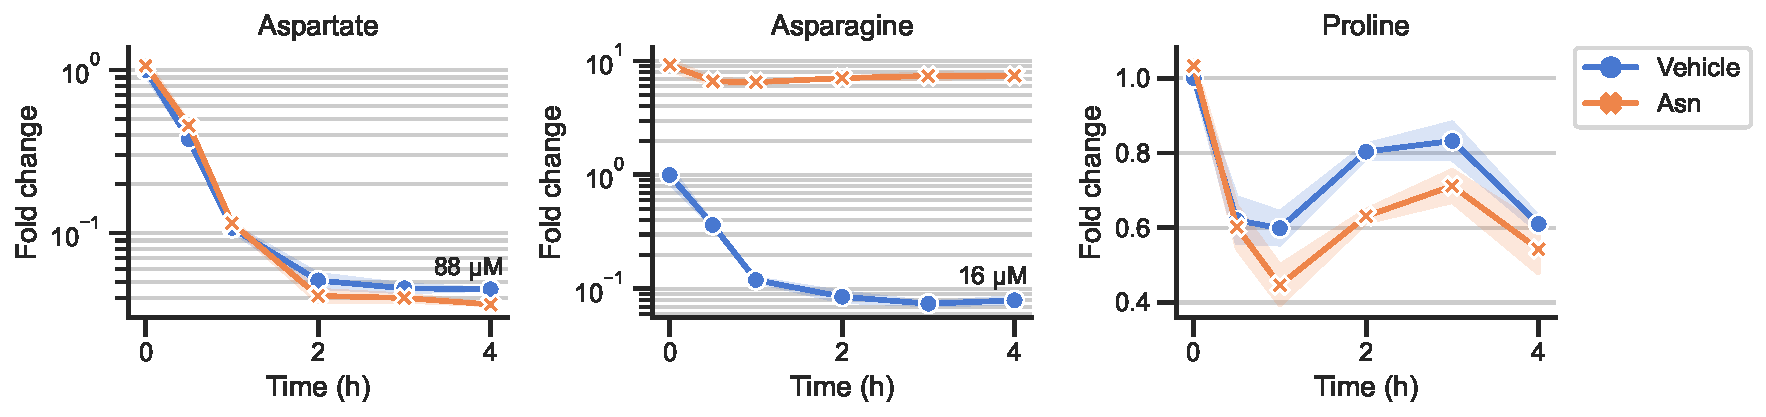
\includegraphics[width=\textwidth]{figures/chap2/app/HT1080_Anti_AA.pdf}
         \caption{Amino acids}
         \label{fig:app_ch2:HT1080_Anti_AA}
     \end{subfigure}
     \hfill
     \begin{subfigure}[b]{0.45\textwidth}
         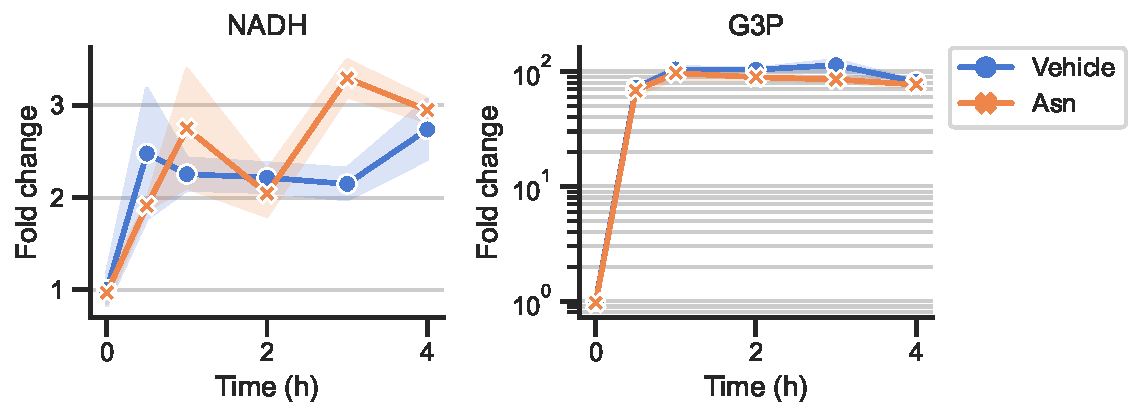
\includegraphics[width=\textwidth]{figures/chap2/app/HT1080_Anti_rd.pdf}
         \caption{Redox metabolites}
         \label{fig:app_ch2:HT1080_Anti_rd}
     \end{subfigure}
     \hfill
     \begin{subfigure}[b]{0.9\textwidth}
         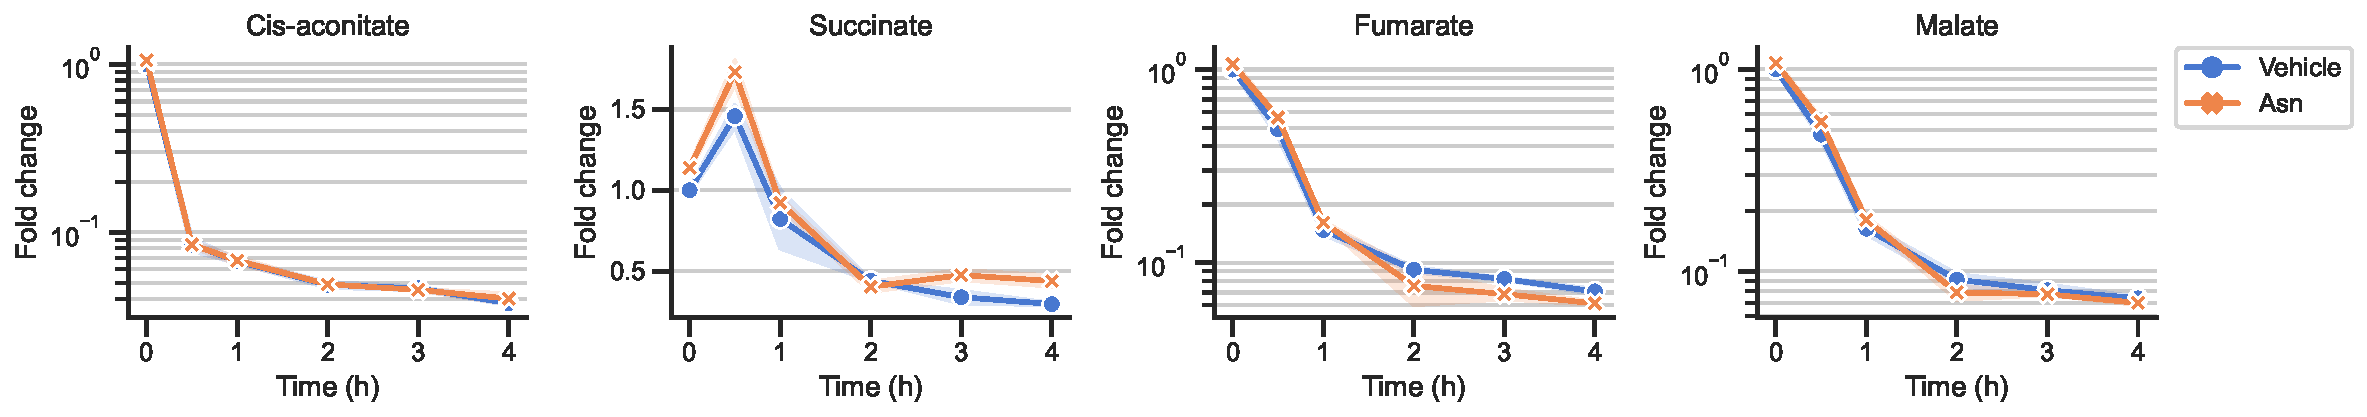
\includegraphics[width=\textwidth]{figures/chap2/app/HT1080_Anti_tca.pdf}
         \caption{TCA metabolites}
         \label{fig:app_ch2:HT1080_Anti_tca}
     \end{subfigure}
     \hfill
     \begin{subfigure}[b]{0.9\textwidth}
         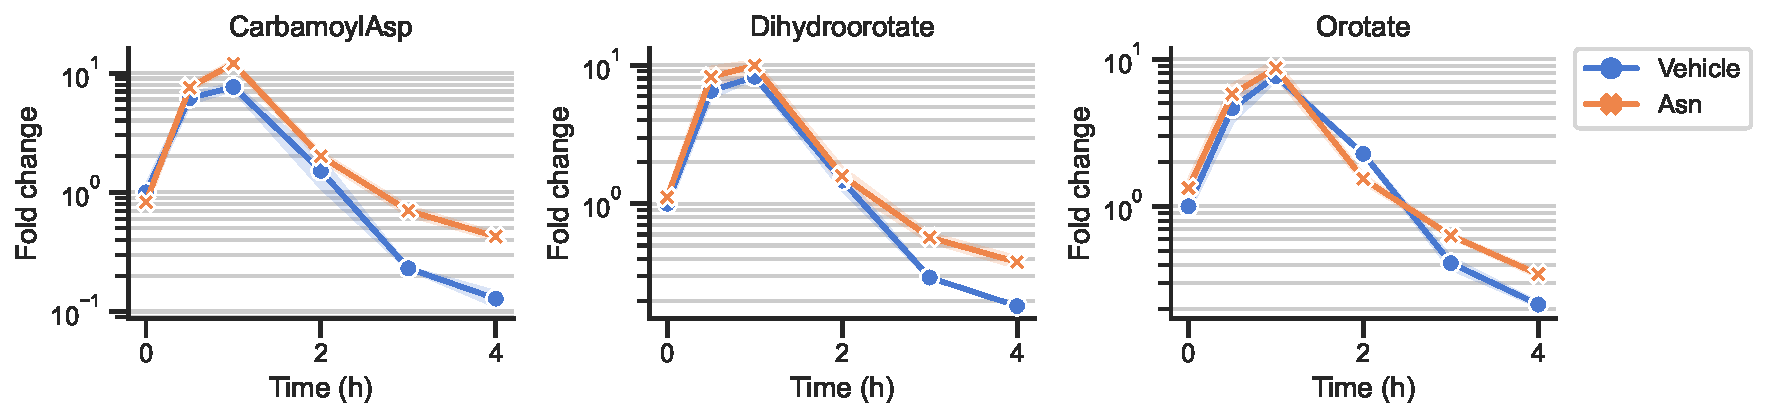
\includegraphics[width=\textwidth]{figures/chap2/app/HT1080_Anti_pyr.pdf}
         \caption{Pyrimidine metabolites}
         \label{fig:app_ch2:HT1080_Anti_pyr}
     \end{subfigure}
     \hfill
     \begin{subfigure}[b]{0.68\textwidth}
         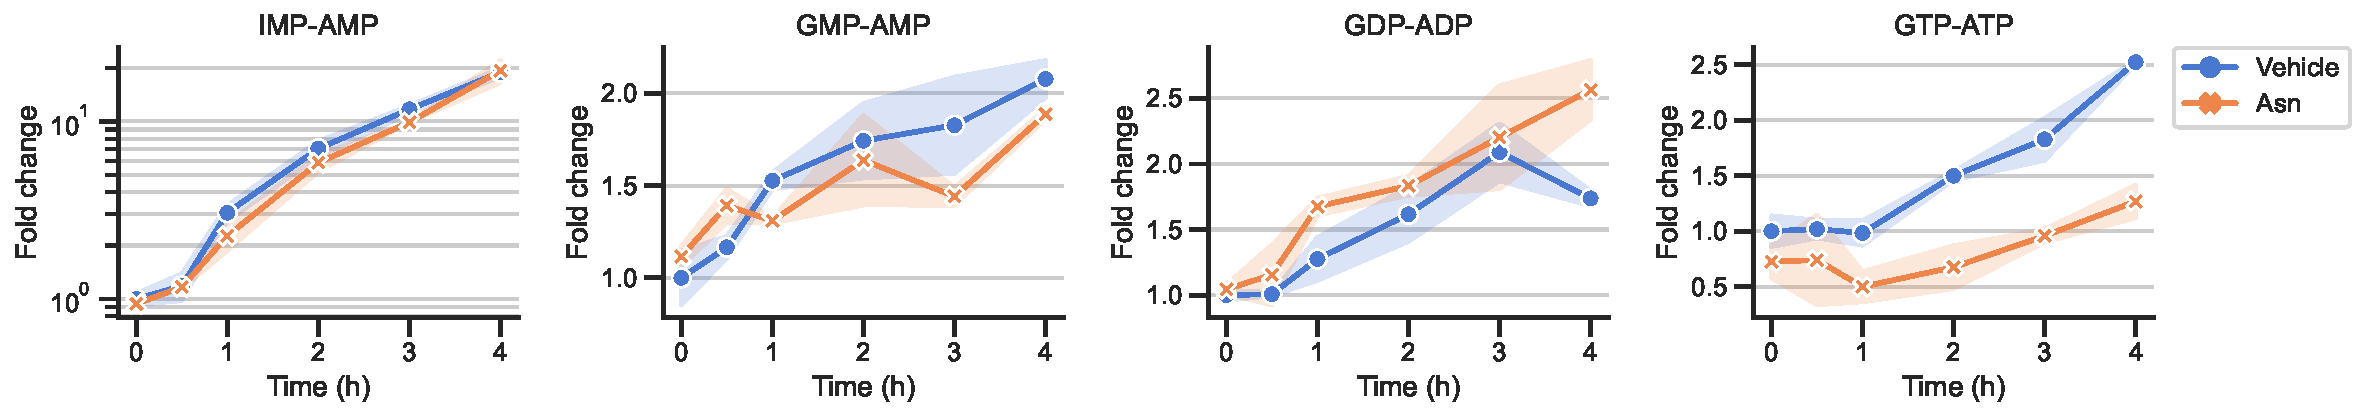
\includegraphics[width=\textwidth]{figures/chap2/app/HT1080_Anti_pur.pdf}
         \caption{Purine metabolites (and dTTP)}
         \label{fig:app_ch2:HT1080_Anti_pur}
     \end{subfigure}
     \hfill
        \caption[Metabolic changes in HT1080 after antimycin treatment]{
        Metabolic changes in HT1080 WT after antimycin (1 µM) treatment.
        From same experiment as figure \ref{fig:ch2:ISR_resc}.
        }
        \label{fig:app_ch2:HT1080_Anti_metab}
\end{figure}



















\begin{figure}
    \centering
    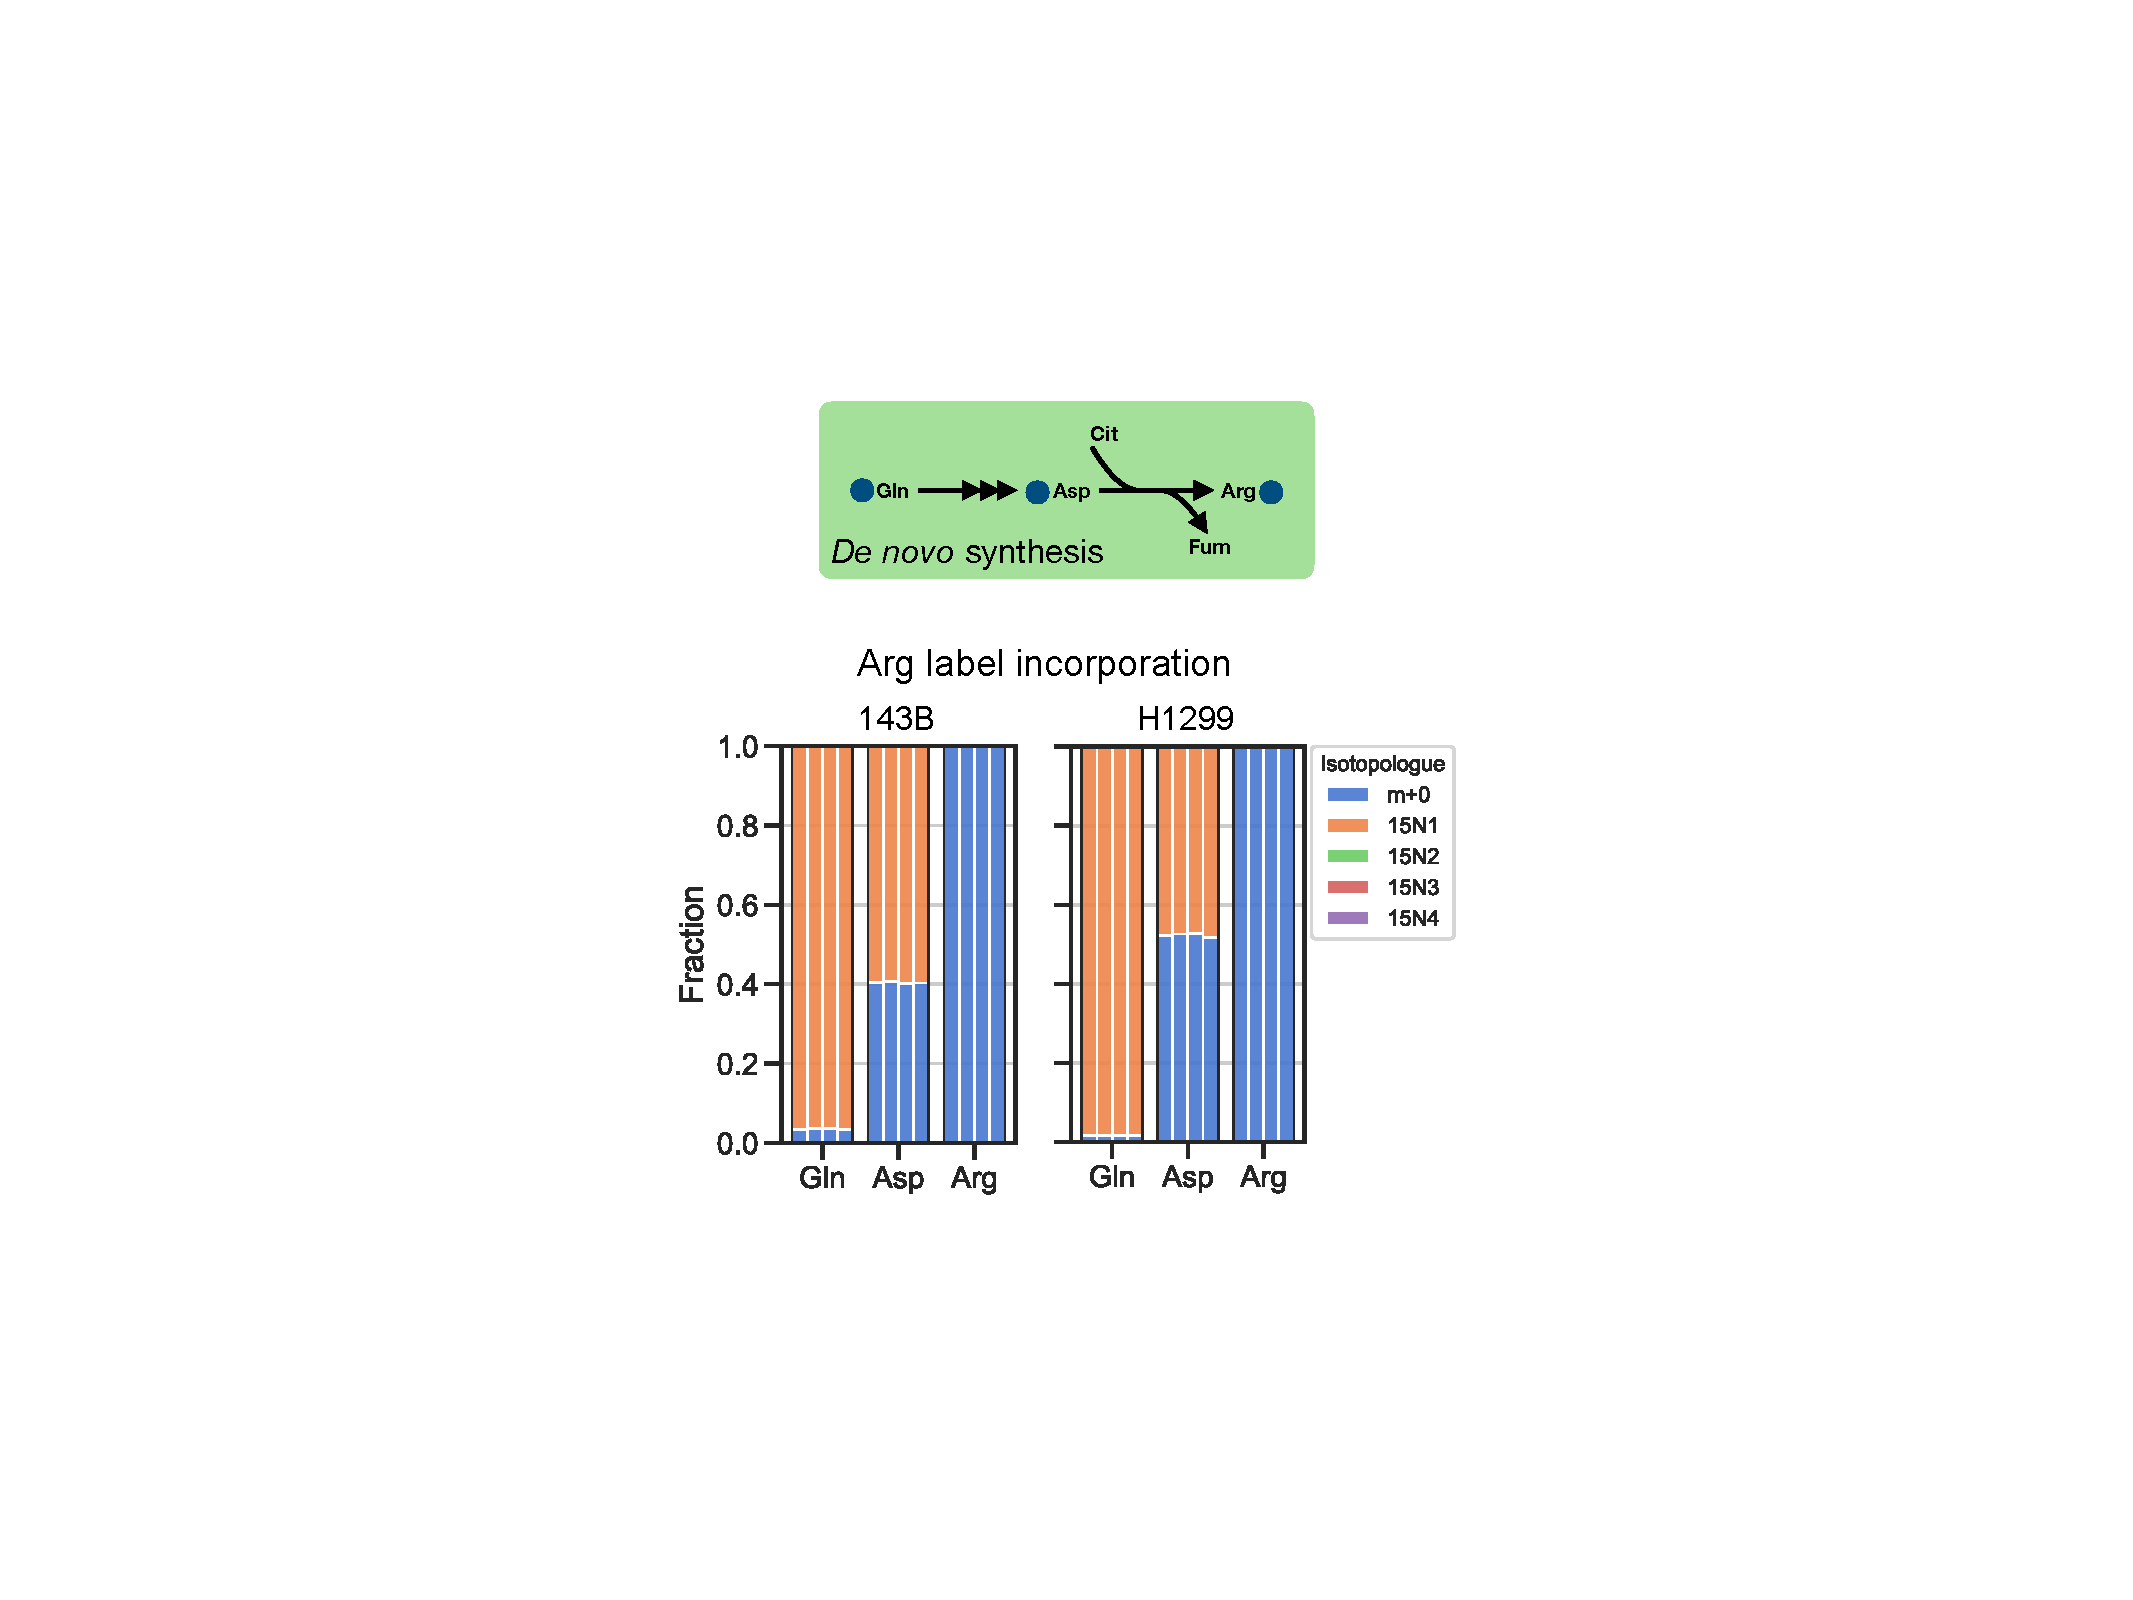
\includegraphics[width=0.45\textwidth]{figures/chap2/app/arg_syn.pdf}
    \caption[No evidence of arginine synthesis in DMEM]{
    No evidence of arginine synthesis in DMEM.
    Top diagram shows Gln alpha\=/\hNi{} label incorporation into Asp and subsequently Arg.
    Bottom isotopologue distribution shows Gln alpha\=/\hNi{} label incorporation into Gln, Asp and Arg at steady-state for cell lines 143B and H1299 grown in DMEM.
    }
    \label{fig:app_ch2:arg_syn}
\end{figure}










\begin{figure}
    \centering
    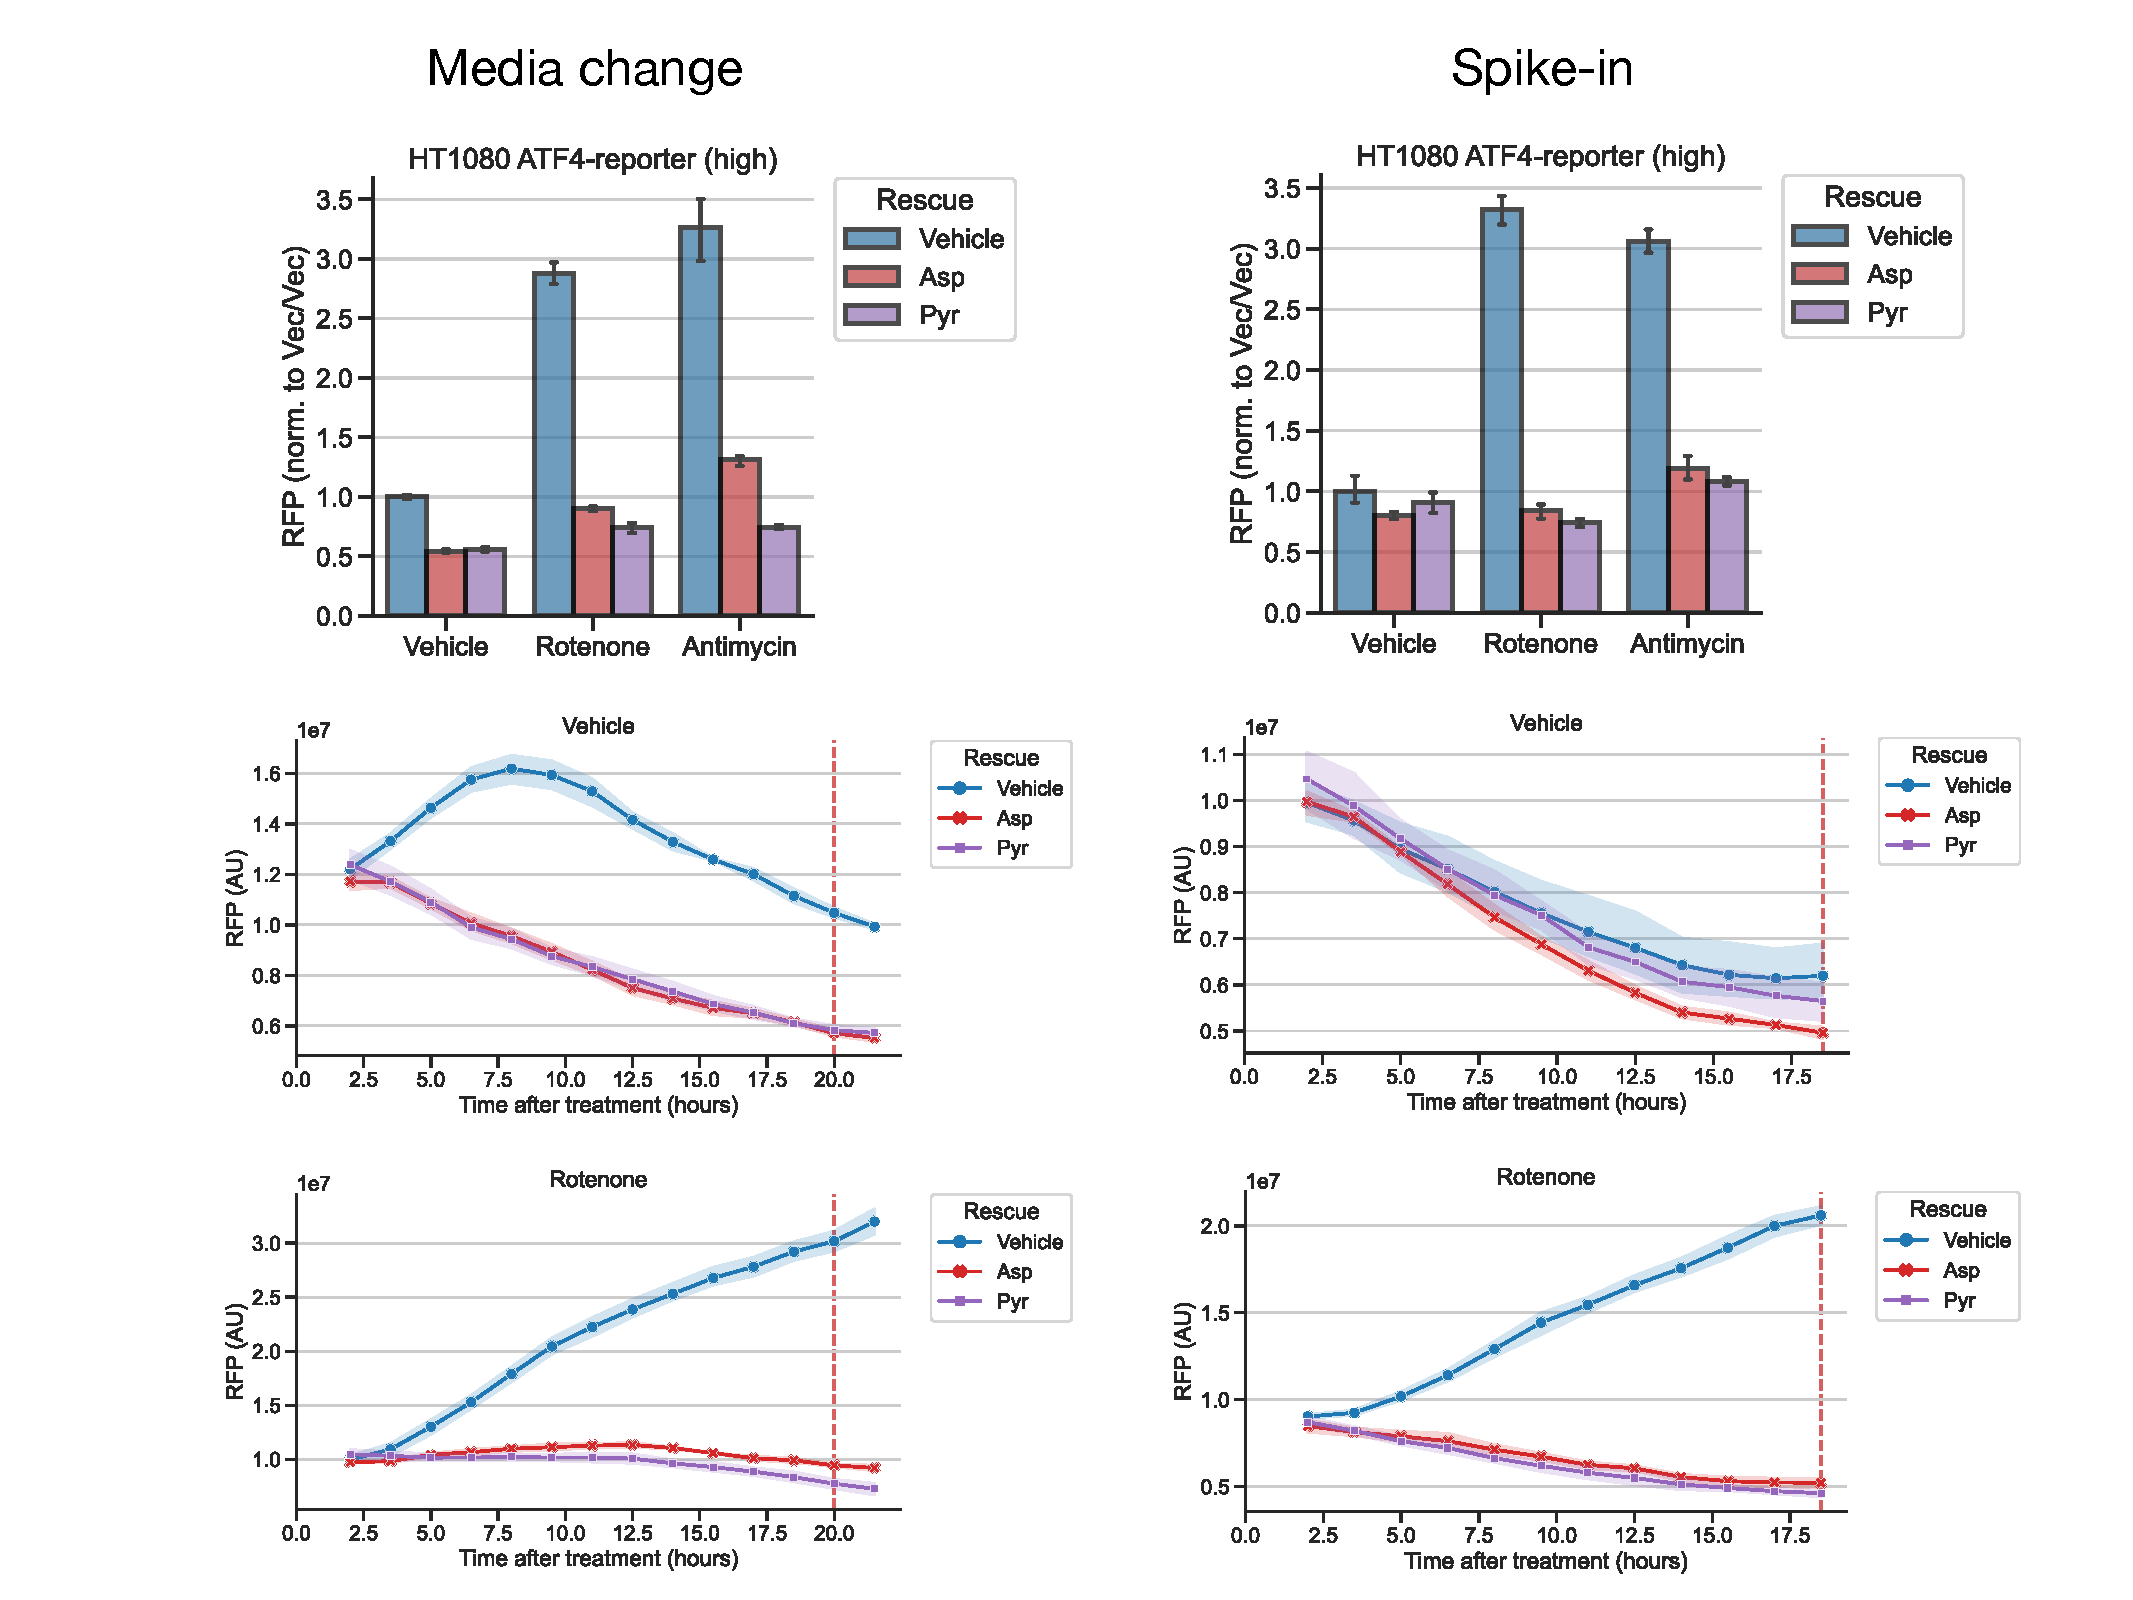
\includegraphics[width=0.95\textwidth]{figures/chap2/app/atf4_chVSsp.pdf}
    \caption[ATF4 reporter, media change vs. spike-in]{
    Mitochondrial inhibitor induced ATF4 reporter, media change vs. spike-in.
    Left column showing results from an experiment were media change was used to initiate the treatment.
    Right column showing results from an experiment were the treatment was initiated by a 10x spike-in.
    Barplots showing results at the time indicated by the red dashed line on the lineplots below.
    }
    \label{fig:app_ch2:sal_frac_conc}
\end{figure}


\begin{figure}
    \centering
    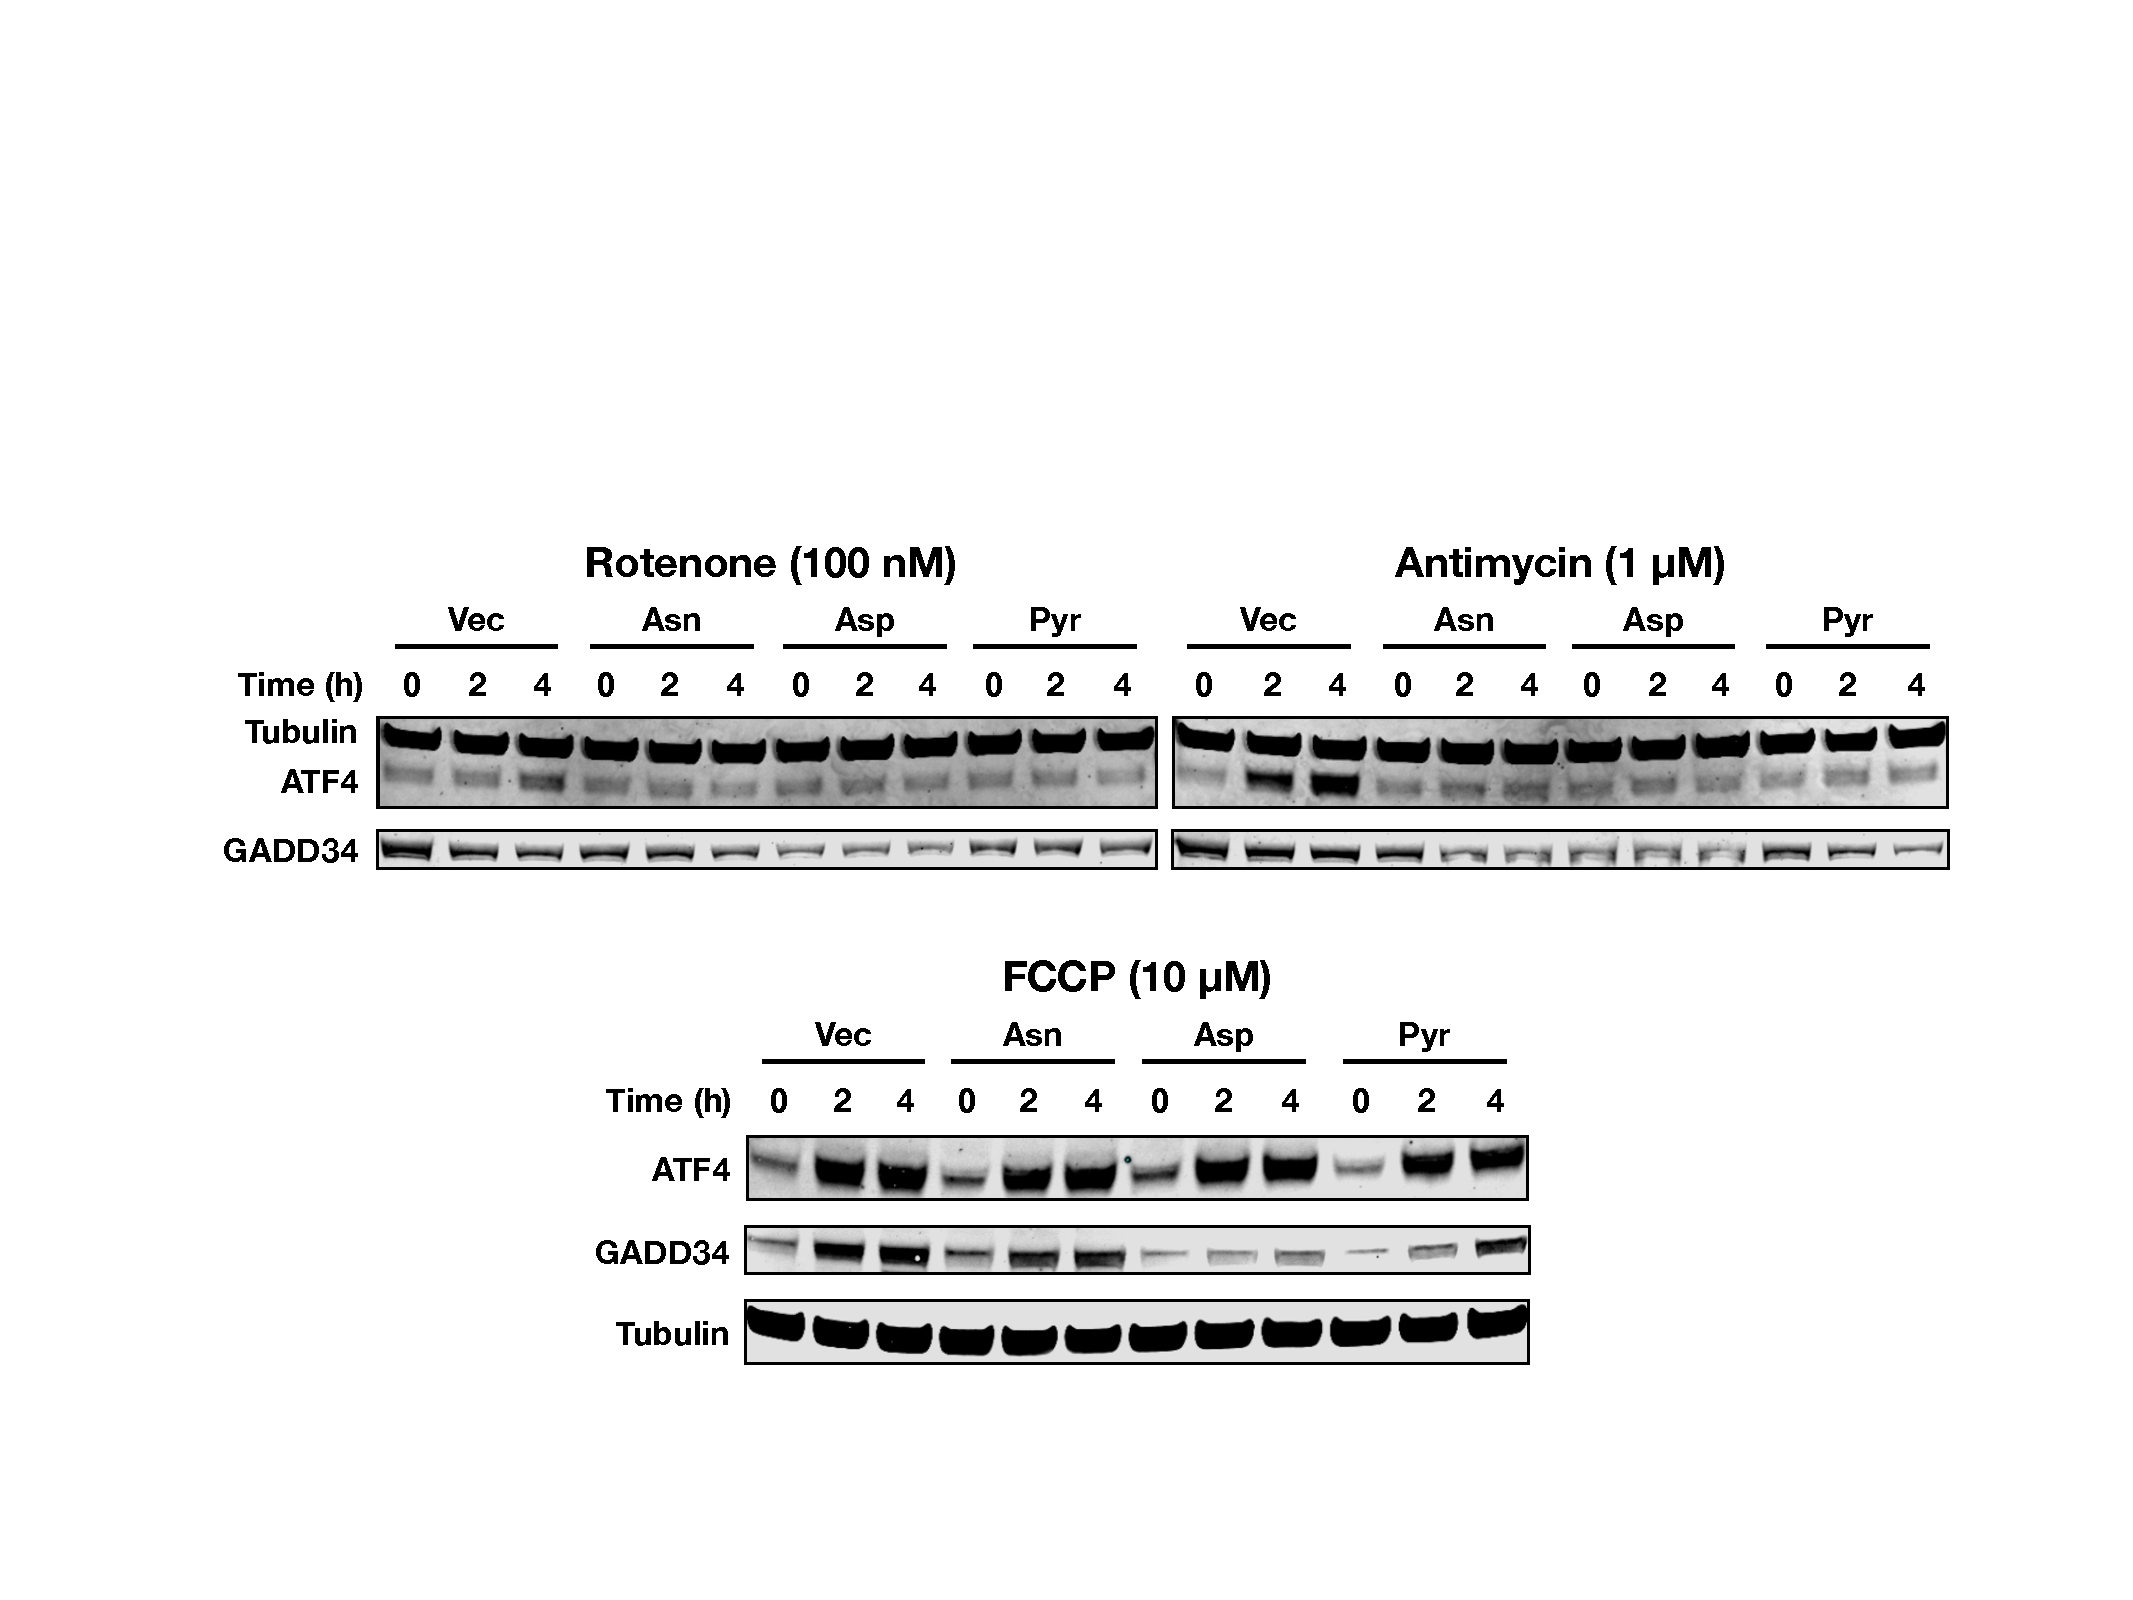
\includegraphics[width=0.95\textwidth]{figures/chap2/app/HT1080_ISR_western.pdf}
    \caption[Mito inhibitor, ATF4 western]{
    Western blot validation of ATF4 reporter in HT1080 cells.
    Treatment and rescue conditions similar to figure \ref{fig:ch2:ISR}.
    % Wednesday 01/12/22
    }
    \label{fig:app_ch2:HT1080_ISR_western}
\end{figure}



\begin{figure}
    \centering
    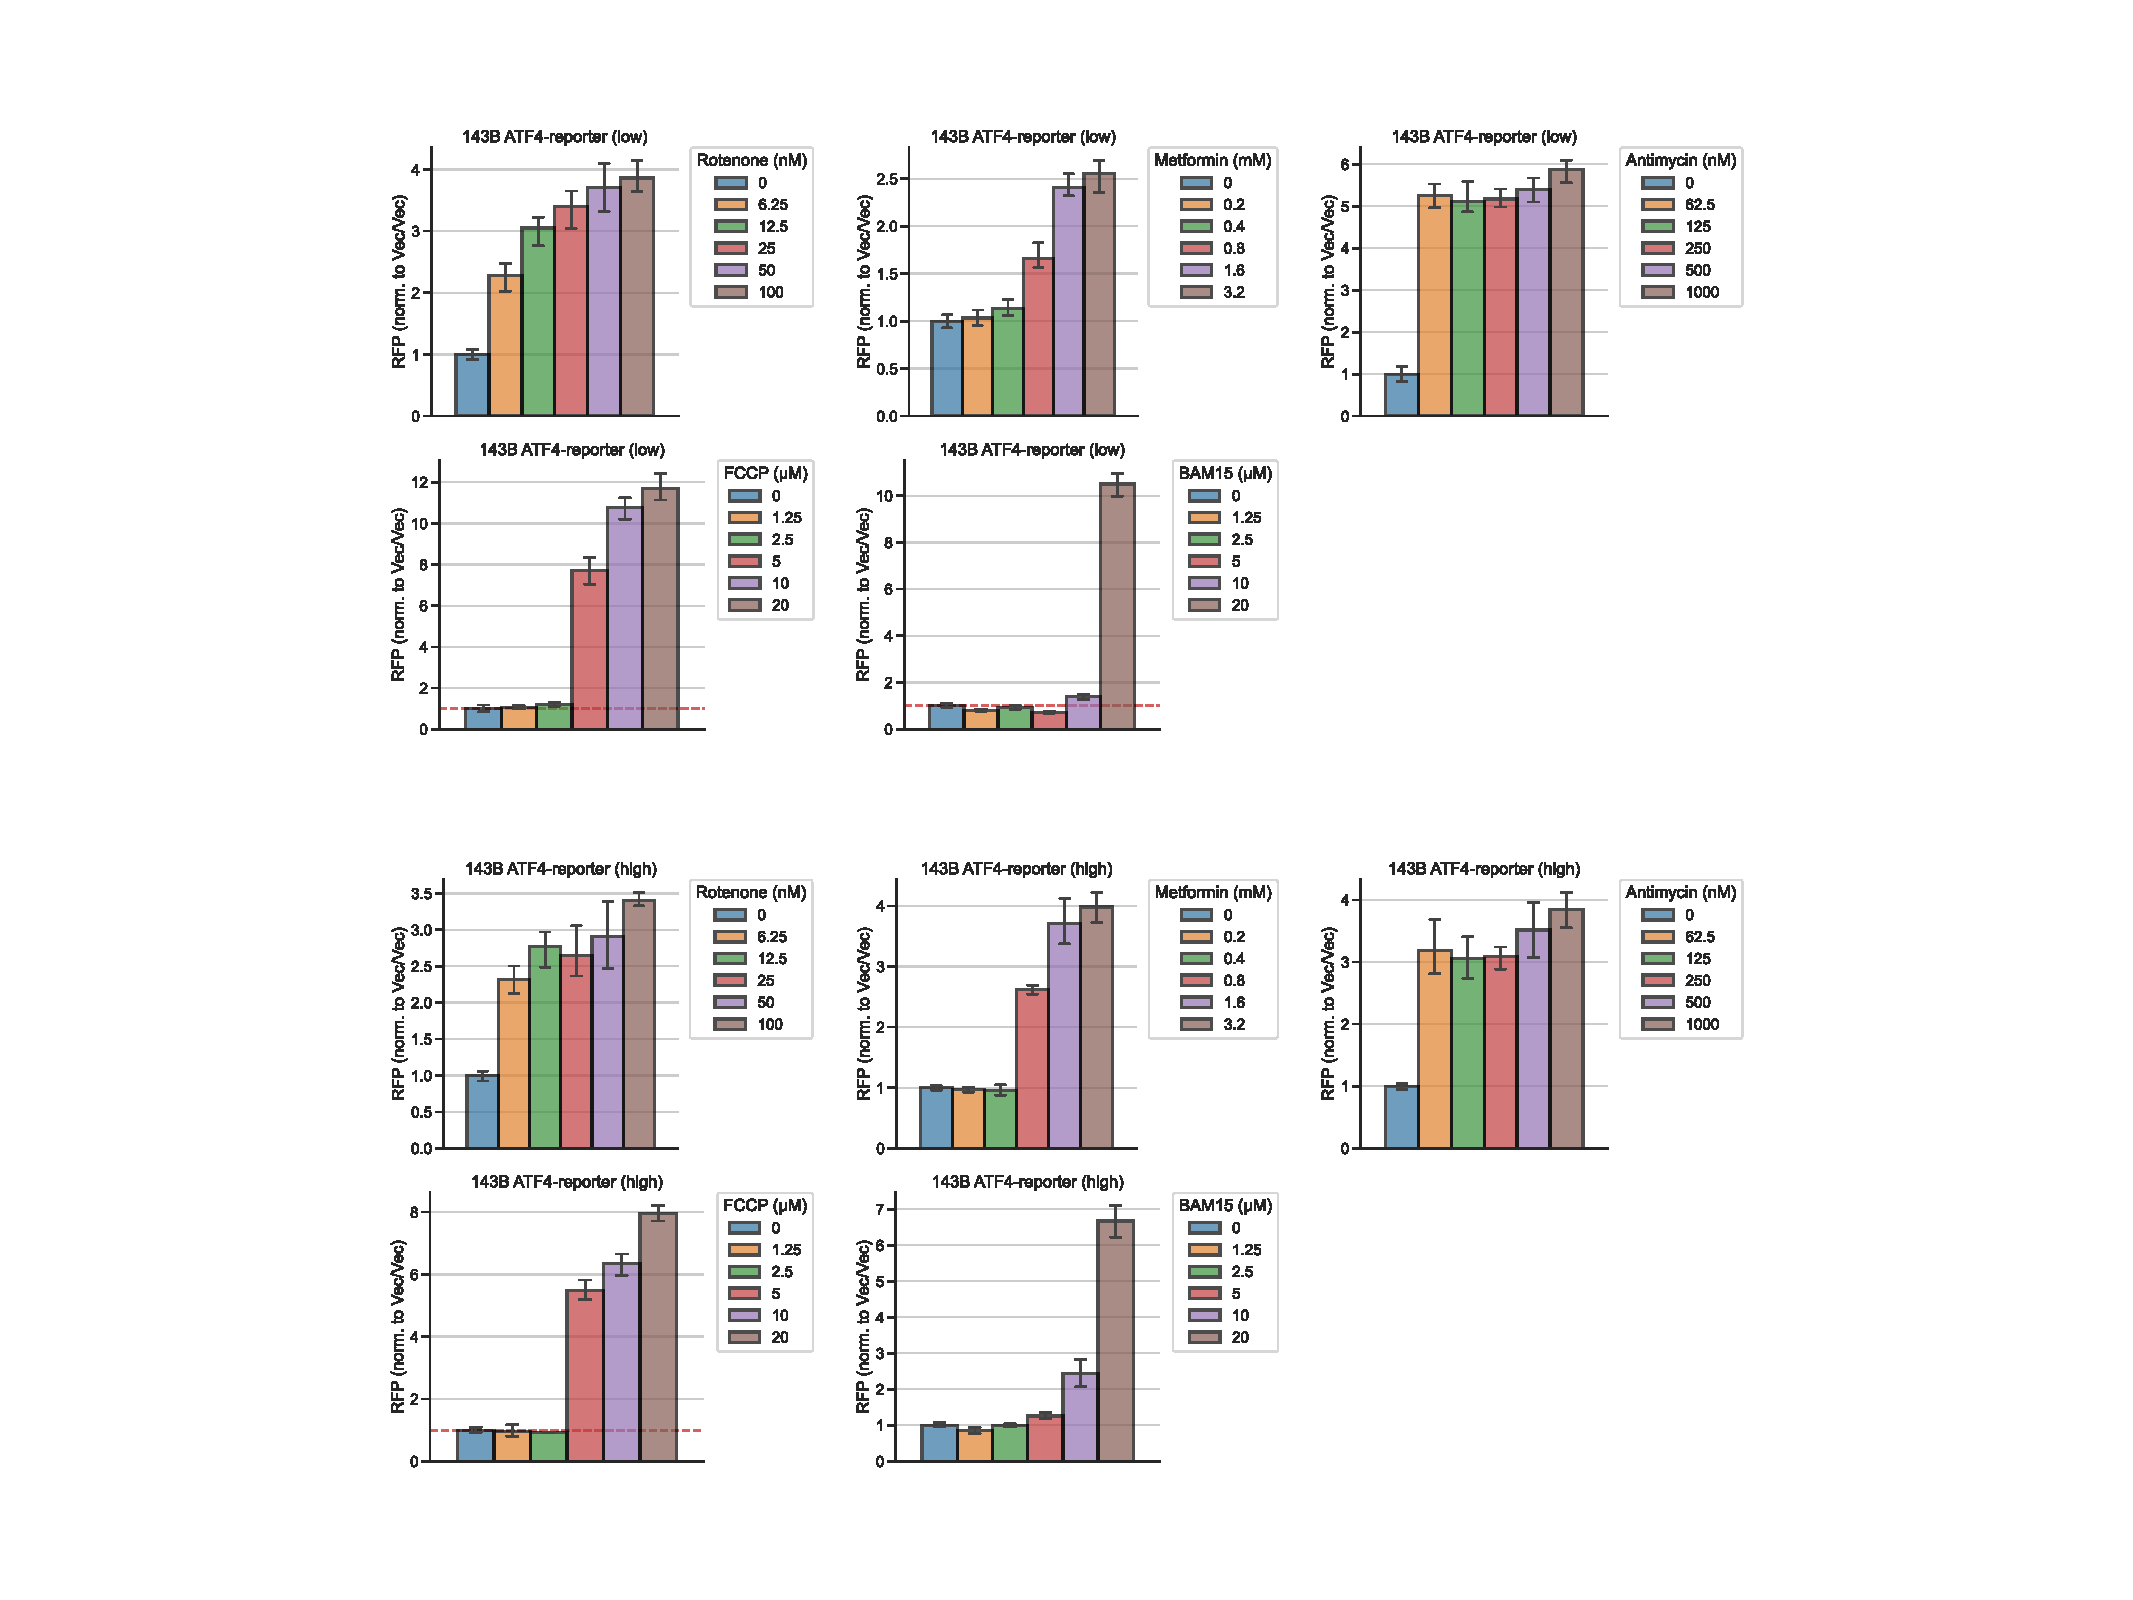
\includegraphics[width=0.95\textwidth]{figures/chap2/app/atf4_ETCtit.pdf}
    \caption[ATF4 reporter, drug titrations]{
    ATF4 reporter, drug titrations.
    ATF4 reporter readout at 17.5 h after drug treatments in 143B cells.
    }
    \label{fig:app_ch2:atf4_ETCtit}
\end{figure}




\begin{figure}
     \centering
     \begin{subfigure}[b]{0.49\textwidth}
         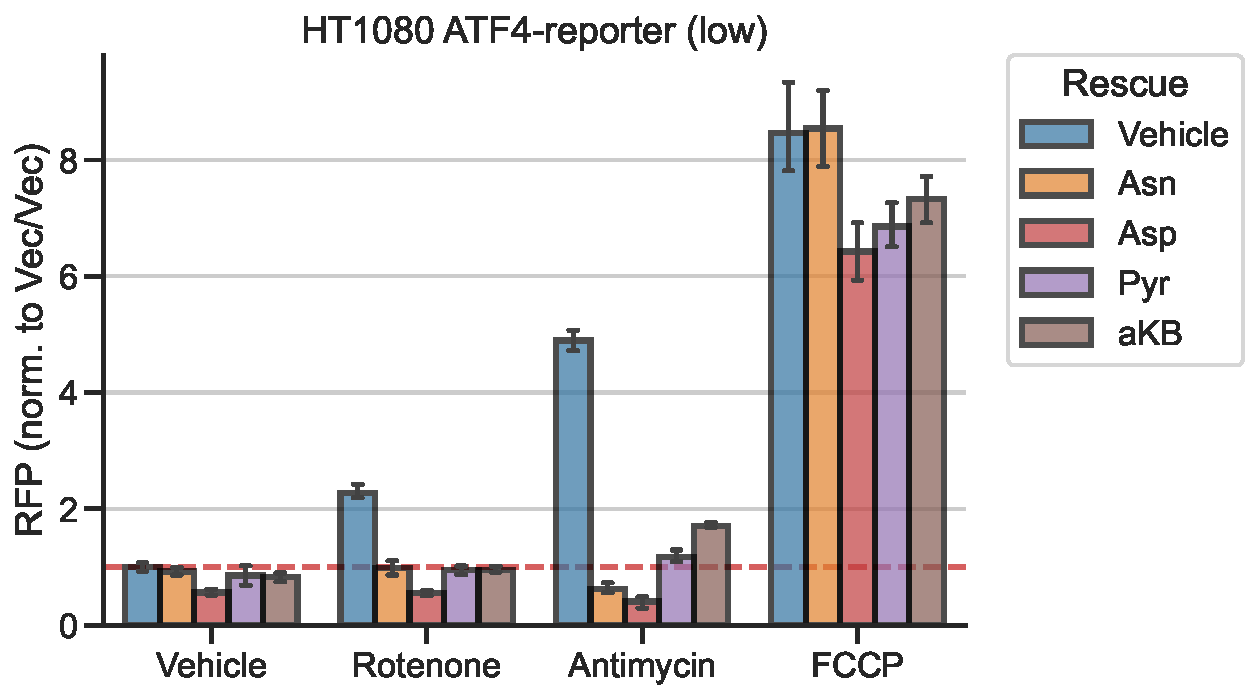
\includegraphics[width=\textwidth]{figures/chap2/app/HT1080_ETCinhib_ATF4rep_low.pdf}
         \caption{}
         \label{fig:app_ch2:HT1080_ETCinhib_ATF4rep_low}
     \end{subfigure}
     \hfill
     \begin{subfigure}[b]{0.49\textwidth}
         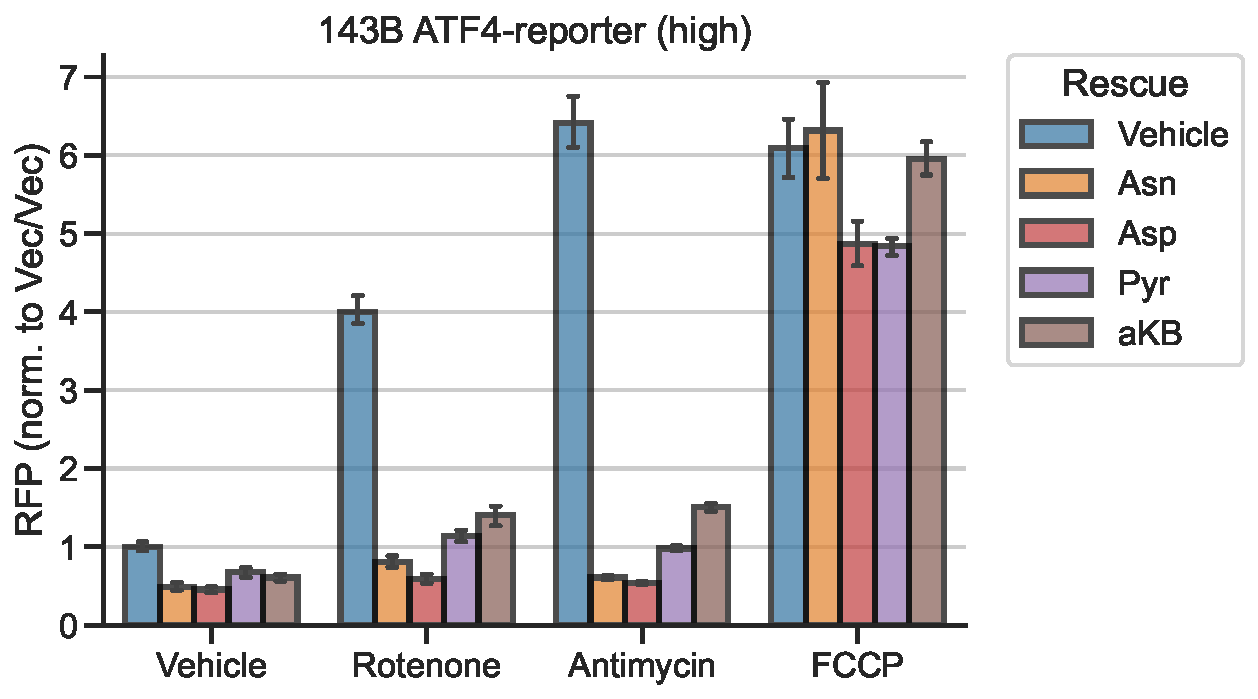
\includegraphics[width=\textwidth]{figures/chap2/app/143B_ETCinhib_ATF4rep_high.pdf}
         \caption{}
         \label{fig:app_ch2:143B_ETCinhib_ATF4rep_high}
     \end{subfigure}
     \hfill
     \begin{subfigure}[b]{0.4\textwidth}
         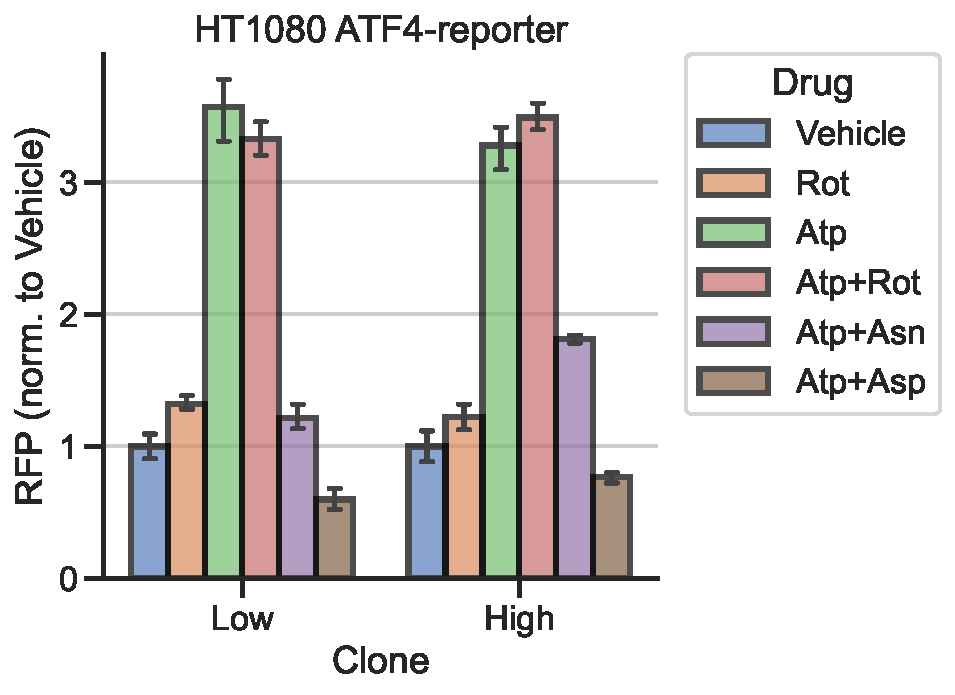
\includegraphics[width=\textwidth]{figures/chap2/app/HT1080_Atp_ATF4rep.pdf}
         \caption{}
         \label{fig:app_ch2:HT1080_Atp_ATF4rep}
     \end{subfigure}
     \hspace{0.06\textwidth}
     \begin{subfigure}[b]{0.4\textwidth}
         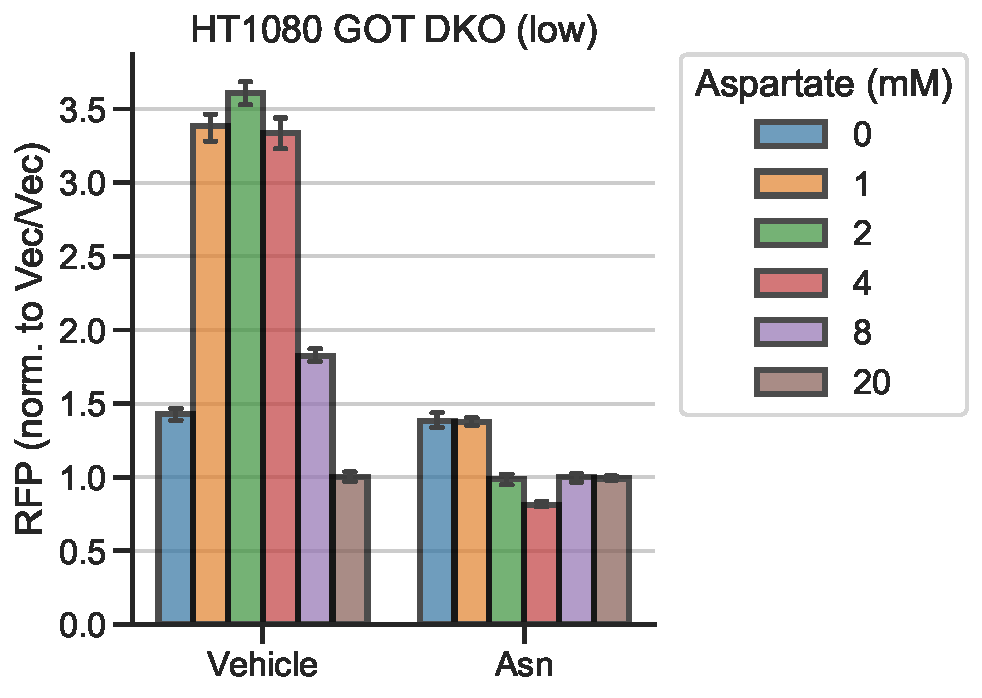
\includegraphics[width=\textwidth]{figures/chap2/app/HT1080_GOT_DKO_Asp_ATF4rep.pdf}
         \caption{}
         \label{fig:app_ch2:HT1080_GOT_DKO_Asp_ATF4rep}
     \end{subfigure}
        \caption[Mito inhibitor induced ATF4 is rescued by Asn, other clones]{
        Related to figure \ref{fig:ch2:ISR}, here showing data generated for other clones.
        (d) Measured 20.5 h after aspartate depletion, Vec/Vec normalization is normalization to the baseline condition (20 mM Asp, no Asn).
        }
        \label{fig:app_ch2:ISR}
\end{figure}




\begin{figure}
    \centering
    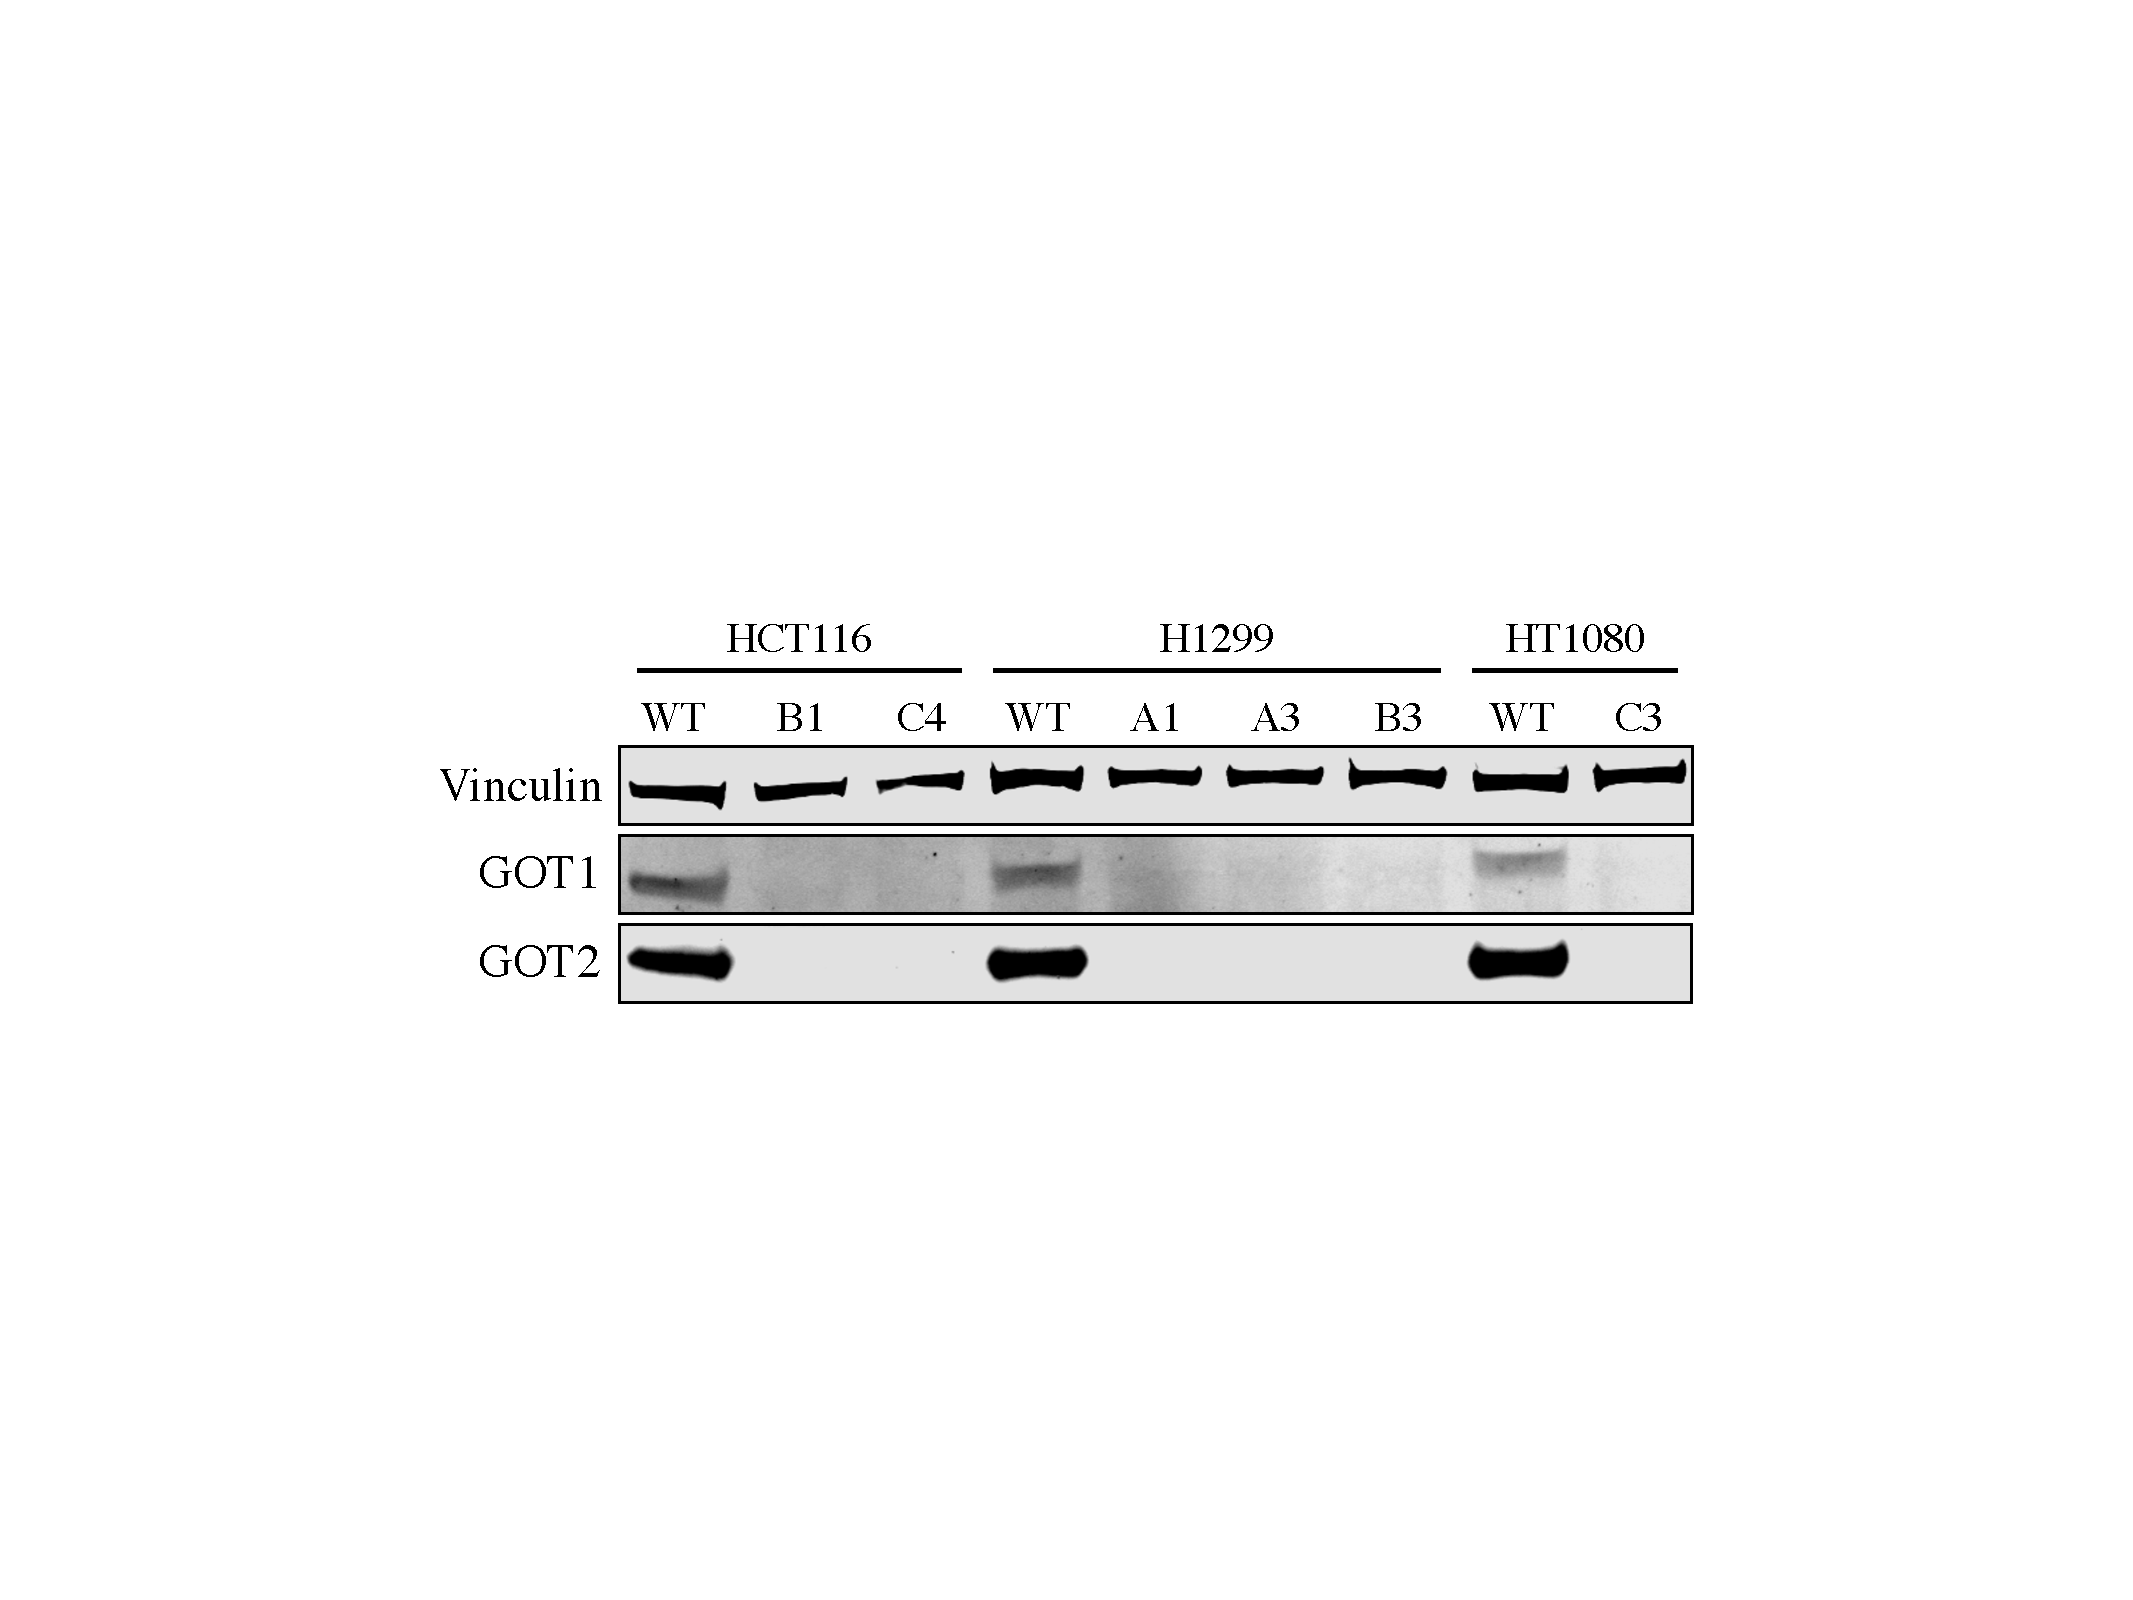
\includegraphics[width=0.55\textwidth]{figures/chap2/app/GOT_DKO_western.pdf}
    \caption[GOT DKO western blot validation]{
    Western blot validation of GOT DKO single cell clones.
    }
    \label{fig:app_ch2:GOT_DKO_western}
\end{figure}








